\subsection{EventProcessing}

\subsubsection*{Results}

All tests are run with the following settings.

Event sources = 3

EventSource.minTimes = [ 10, 20, 30, 40, 50, 10, 20, 30, 40 ]

EventSource.maxTimes = [ 100, 150, 200, 50, 60, 30, 60, 100, 80 ]

EventProcessing.minTime = 10

EventProcessing.maxTime = 400

\textbf{Test 1 - FairMultiplex}

\begin{tabular}{c|c}

	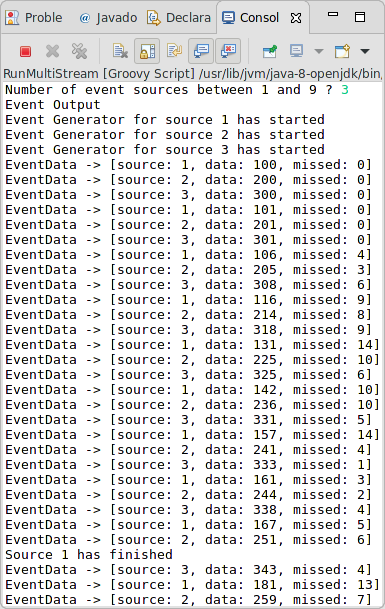
\includegraphics[width=\textwidth/2]{img/screenshots/9-3-1-1.png} &
	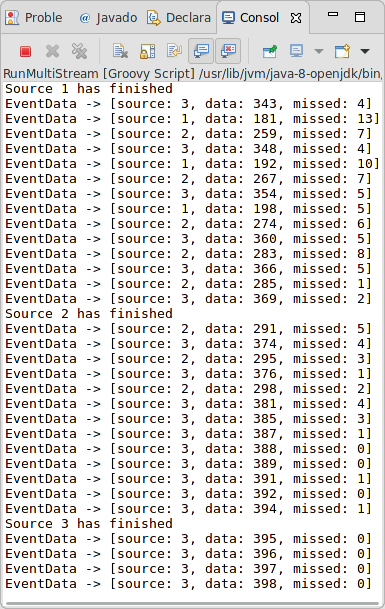
\includegraphics[width=\textwidth/2]{img/screenshots/9-3-1-2.png} \\

\end{tabular}

\textbf{Test 2 - PriMultiplex}

\begin{tabular}{c|c}

	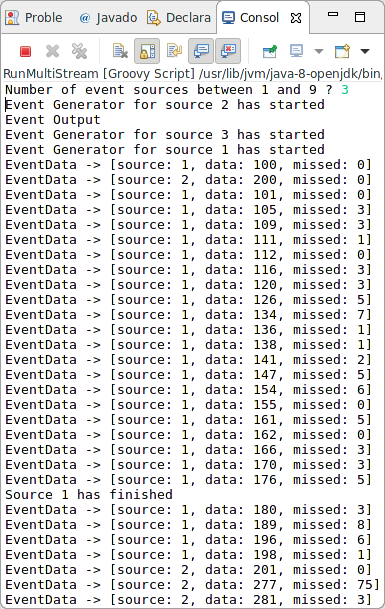
\includegraphics[width=\textwidth/2]{img/screenshots/9-3-2-1.png} &
	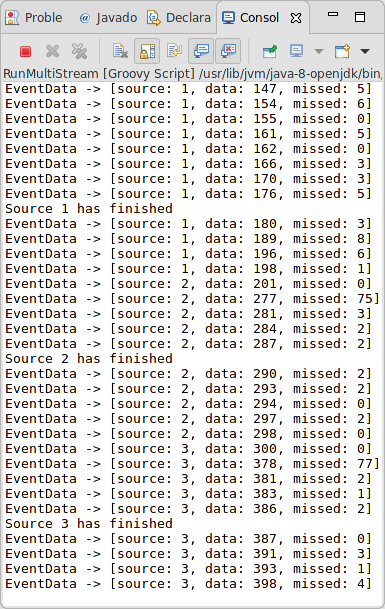
\includegraphics[width=\textwidth/2]{img/screenshots/9-3-2-2.png} \\

\end{tabular}

\textbf{Test 3 - Multiplex}

\begin{tabular}{c|c}

	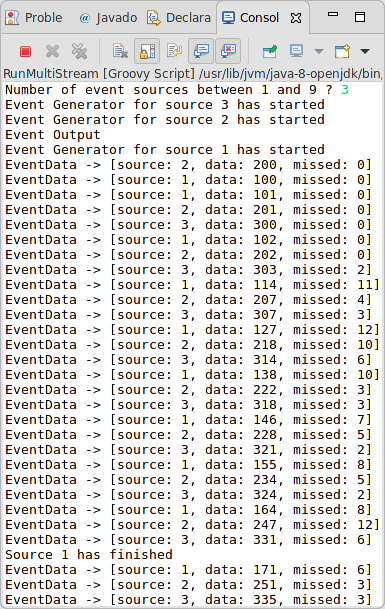
\includegraphics[width=\textwidth/2]{img/screenshots/9-3-3-1.png} &
	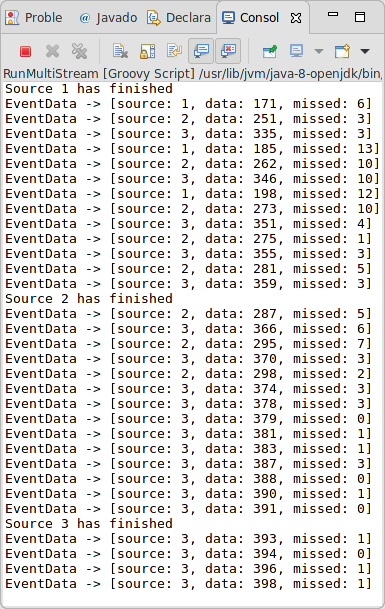
\includegraphics[width=\textwidth/2]{img/screenshots/9-3-3-2.png} \\

\end{tabular}

\subsubsection*{Conclusion}

\paragraph{Test 1} shows that each source is read from in order.  This however has the effect of causing the earlier resources to have a greater quantity of missed data as can be seen by source 1 finishing before source 2 and source 2 finishing before source 3.

\paragraph{Test 2} shows that source one is ready from until there is no data left to be read, then source two and finally source three.  This results in source 1 having very little missed data, however source two and three miss 75 and 77 data elements respectively after the first element of each is read.  Source one is always read as it is queued in the EventPrompter.

\paragraph{Test 3} shows a very similar result to test 1 however test one waits for each source to begin generating events before reading the second data element form source 1.  This means that in a system where events were not generated equally test 3 would significantly outperform test 1.
